\documentclass[11pt]{article}

% ---------------------------------------------------------------------------
%  spatial_prognosis -- SRI Research Proposal
%  Compile with:  tectonic docs/proposal.tex
% ---------------------------------------------------------------------------

\usepackage[margin=1in]{geometry}
\usepackage{amsmath,amssymb}
\usepackage{xcolor}
\usepackage{tikz}
\usetikzlibrary{arrows.meta,positioning,fit,backgrounds,calc,shapes.geometric}
\usepackage{booktabs}
\usepackage{array}
\usepackage{colortbl}
\usepackage[most]{tcolorbox}
\usepackage{enumitem}
\usepackage{graphicx}
\usepackage[colorlinks=true,linkcolor=sriblue,citecolor=sriblue,urlcolor=sriaccent]{hyperref}

\definecolor{sriblue}{HTML}{1F4E79}
\definecolor{sriaccent}{HTML}{E8684A}
\definecolor{srigreen}{HTML}{2E8B57}
\definecolor{srigray}{HTML}{4B5563}
\definecolor{srilight}{HTML}{EAF1F8}
\definecolor{srirow}{HTML}{F2F6FB}
\definecolor{cTumor}{HTML}{5B8FF9}
\definecolor{cImmune}{HTML}{E8684A}

\usepackage{titlesec}
\titleformat{\section}{\large\bfseries\color{sriblue}}{\thesection}{0.6em}{}
\titleformat{\subsection}{\normalsize\bfseries\color{sriblue!85!black}}{\thesubsection}{0.5em}{}
\titlespacing*{\section}{0pt}{1.4ex}{0.8ex}

\newtcolorbox{problembox}{colback=srilight,colframe=sriblue,boxrule=0.9pt,arc=2pt,left=6pt,right=6pt,top=5pt,bottom=5pt}
\newtcolorbox{gapbox}{colback=sriaccent!8,colframe=sriaccent,boxrule=0.9pt,arc=2pt,left=6pt,right=6pt,top=5pt,bottom=5pt}
\newtcolorbox{aimbox}[1]{colback=srigreen!7,colframe=srigreen,boxrule=0.8pt,arc=2pt,left=6pt,right=6pt,top=4pt,bottom=4pt,title={#1},fonttitle=\bfseries\color{white},colbacktitle=srigreen}

\renewcommand{\arraystretch}{1.25}
\newcommand{\NN}{\mathcal{N}}

\begin{document}

\begin{center}
  {\LARGE\bfseries\color{sriblue} Does the Spatial Architecture of a Tumor\\ Predict Patient Outcome?}\\[3pt]
  {\large\bfseries\color{sriblue!80!black} Testing whether \emph{where} immune cells sit -- not just \emph{how many} --\\ carries prognostic signal, with a spatial graph neural network}\\[10pt]
  {\large Akshatha Arunkumar}\\[2pt]
  {\small Student Research Institute (SRI) -- Summer 2026 Cohort \\
  Harvard Undergraduate OpenBio Laboratory}\\[2pt]
  {\small\itshape Research Proposal for Mentor Review \quad\textbar\quad \today}
\end{center}

\vspace{2pt}
\begin{problembox}
\textbf{The problem.} Whether a cancer patient does well often depends not just
on \emph{which} cells are in their tumor but on \emph{how those cells are
spatially arranged} -- in particular, whether immune cells \emph{infiltrate} the
tumor (often favorable) or are \emph{excluded} from it (often unfavorable). Two
tumors can have the \emph{identical} cell composition yet opposite outcomes
because of this arrangement. Standard analyses summarize a tumor by its cell
\emph{proportions} and therefore cannot see this. This project asks, rigorously:
\textbf{does the spatial arrangement of the tumor microenvironment add
prognostic signal beyond composition?}
\end{problembox}

% ===========================================================================
\section{Background and Significance}

The tumor microenvironment (TME) -- the ecosystem of tumor, immune, and stromal
cells -- is a central determinant of cancer progression and response to therapy.
A growing body of pathology shows that the \emph{spatial organization} of this
ecosystem is prognostic: ``immune-inflamed'' tumors with cytotoxic T cells in
contact with tumor cells tend to respond better than ``immune-excluded'' tumors
where those same T cells are trapped at the margin. New technologies (imaging
mass cytometry, CODEX, spatial transcriptomics) now measure dozens of markers
per cell \emph{while preserving each cell's location}, making it possible to
quantify TME architecture at single-cell resolution.

\begin{table}[h]
\centering\small
\begin{tabular}{>{\raggedright\arraybackslash}p{0.30\linewidth} >{\raggedright\arraybackslash}p{0.62\linewidth}}
\toprule
\rowcolor{sriblue}\color{white}\textbf{Why it matters} & \color{white}\textbf{Consequence}\\
\midrule
\rowcolor{srirow} Outcome depends on cell \emph{arrangement} & Two tumors with the same composition can have opposite prognoses.\\
Composition summaries discard geometry & Proportion-based models are blind to infiltration vs.\ exclusion.\\
\rowcolor{srirow} Spatial single-cell data now exist & We can finally test the arrangement hypothesis directly.\\
\bottomrule
\end{tabular}
\caption{Spatial arrangement of the TME is widely believed prognostic; testing
whether it adds signal beyond composition is the question we address.}
\label{tab:significance}
\end{table}

% ===========================================================================
\section{The Unmet Need}

\begin{gapbox}
\textbf{Gap 1 -- Composition hides geometry.} Summarizing a tumor by its cell
proportions cannot distinguish an infiltrated tumor from an excluded one with
the same cell counts.\\[3pt]
\textbf{Gap 2 -- Most spatial models \emph{assume} arrangement matters.} Many
TME outcome models report accuracy without isolating whether the gain comes from
spatial structure or merely from composition -- so the central biological claim
is rarely tested.
\end{gapbox}

\noindent We close Gap 2 with a controlled, falsifiable comparison
(Fig.~\ref{fig:mechanism}): a model that reads spatial arrangement vs.\ strong
composition-only models, plus an ablation that destroys the arrangement.

\begin{figure}[h]
\centering
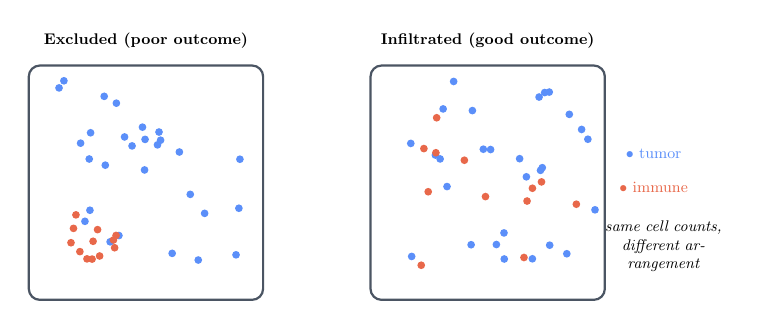
\begin{tikzpicture}[scale=0.62,every node/.style={transform shape}]
  % two panels: excluded (left) vs infiltrated (right), SAME counts
  \foreach \cx/\lab/\mode in {0/{Excluded (poor outcome)}/0, 7/{Infiltrated (good outcome)}/1}{
    \draw[rounded corners,draw=srigray,thick] (\cx-0.4,-0.4) rectangle (\cx+4.4,4.4);
    \node[font=\small\bfseries] at (\cx+2,4.9) {\lab};
    \foreach \i in {1,...,28}{
      \pgfmathsetmacro{\px}{\cx+0.2+4.0*rnd}
      \pgfmathsetmacro{\py}{0.2+4.0*rnd}
      \node[circle,fill=cTumor,minimum size=4.5pt,inner sep=0pt] at (\px,\py) {};
    }
    \ifnum\mode=0
      \foreach \i in {1,...,12}{ % immune clustered in a corner (excluded)
        \pgfmathsetmacro{\px}{\cx+0.3+1.1*rnd}
        \pgfmathsetmacro{\py}{0.3+1.1*rnd}
        \node[circle,fill=cImmune,minimum size=4.5pt,inner sep=0pt] at (\px,\py) {};
      }
    \else
      \foreach \i in {1,...,12}{ % immune dispersed (infiltrated)
        \pgfmathsetmacro{\px}{\cx+0.2+4.0*rnd}
        \pgfmathsetmacro{\py}{0.2+4.0*rnd}
        \node[circle,fill=cImmune,minimum size=4.5pt,inner sep=0pt] at (\px,\py) {};
      }
    \fi
  }
  \node[font=\small,cTumor] at (12.4,2.6) {$\bullet$ tumor};
  \node[font=\small,cImmune] at (12.4,1.9) {$\bullet$ immune};
  \node[font=\small,align=center,text width=2.6cm] at (12.6,0.7) {\itshape same cell counts, different arrangement};
\end{tikzpicture}
\caption{Identical composition, opposite arrangement. Composition-only models
see the two tumors as the same; a spatial model reads the tumor--immune contact
structure that distinguishes them.}
\label{fig:mechanism}
\end{figure}

% ===========================================================================
\section{Research Aims}

\begin{aimbox}{Aims}
\textbf{Aim 1.} Represent each patient's tumor as a spatial cell graph and
predict a clinical outcome (tumor grade and/or survival) with a graph neural
network.\\
\textbf{Aim 2.} Test \emph{honestly} whether spatial arrangement adds signal
\emph{beyond composition} -- compare against tuned composition-only baselines
(XGBoost/MLP on cell proportions) and a graph-shuffle ablation.\\
\textbf{Aim 3.} Interpret which spatial cell-neighbourhoods drive prognosis
(candidate prognostic niches), grounding predictions in TME biology.
\end{aimbox}

\noindent\textbf{Guiding questions.} (Q1) Can outcome be predicted from TME
spatial structure? (Q2) Does it beat a composition-only model, and is the gain
\emph{causally} due to arrangement? (Q3) Which spatial niches are prognostic?

% ===========================================================================
\section{Data}

\begin{table}[h]
\centering\small
\begin{tabular}{>{\raggedright\arraybackslash}p{0.27\linewidth} >{\raggedright\arraybackslash}p{0.41\linewidth} >{\raggedright\arraybackslash}p{0.24\linewidth}}
\toprule
\rowcolor{sriblue}\color{white}\textbf{Resource} & \color{white}\textbf{Content} & \color{white}\textbf{Role}\\
\midrule
\rowcolor{srirow} Jackson-Fischer breast IMC & $\sim$700 patients, 37 markers, single-cell coords; tumor grade + survival & Real cohort (primary)\\
METABRIC IMC & 483 tumors, clinical outcomes & External validation\\
\rowcolor{srirow} Controlled synthetic cohort & infiltration vs.\ exclusion, composition matched & Mechanism proof / ablation\\
\bottomrule
\end{tabular}
\caption{All inputs are public, de-identified. Coordinates enter only through
the spatial graph, never as features.}
\label{tab:data}
\end{table}

% ===========================================================================
\section{Proposed Methodology}

Each patient's tumor is a graph: nodes are cells (features = cell-type / marker
profile), edges connect spatially neighbouring cells. We pose outcome prediction
as \textbf{graph classification}.

\subsection{Proposed model: a spatial GNN}
A GraphSAGE/GIN encoder pools each cell's neighbourhood over $L$ hops, then a
global readout summarizes the whole tumor:
\begin{equation}
h_v^{(l)} = \sigma\!\Big(W^{(l)}\big[h_v^{(l-1)}\,\big\Vert\,
\textstyle\operatorname*{AGG}_{u\in\NN(v)} h_u^{(l-1)}\big]\Big), \quad
\hat{y} = \operatorname{softmax}\!\big(\mathrm{MLP}(\textstyle\operatorname*{POOL}_v h_v^{(L)})\big).
\label{eq:gnn}
\end{equation}
The readout depends on neighbourhood structure (e.g.\ tumor--immune contacts),
so the model can represent arrangement, not just composition.

\begin{figure}[h]
\centering
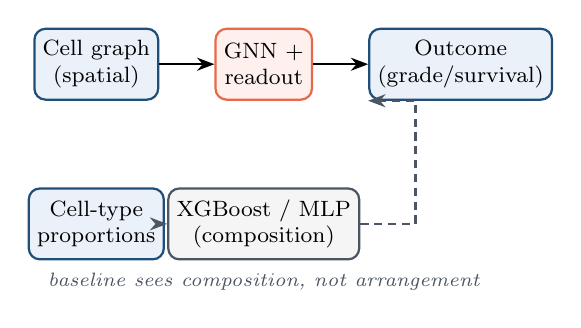
\begin{tikzpicture}[node distance=6mm and 7mm,
  box/.style={rounded corners,draw=sriblue,fill=srilight,thick,minimum height=0.9cm,align=center,font=\footnotesize,inner sep=3pt},
  red/.style={rounded corners,draw=sriaccent,fill=sriaccent!10,thick,minimum height=0.9cm,align=center,font=\footnotesize,inner sep=3pt},
  gray/.style={rounded corners,draw=srigray,fill=gray!8,thick,minimum height=0.9cm,align=center,font=\footnotesize,inner sep=3pt},
  >={Stealth[length=2.2mm]}]
  \node[box] (g) {Cell graph\\(spatial)};
  \node[red,right=of g] (enc) {GNN +\\readout};
  \node[box,right=of enc] (s) {Outcome\\(grade/survival)};
  \draw[->,thick] (g)--(enc); \draw[->,thick] (enc)--(s);
  \node[gray,below=11mm of enc] (mlp) {XGBoost / MLP\\(composition)};
  \node[box,below=11mm of g] (xf) {Cell-type\\proportions};
  \draw[->,thick,densely dashed,srigray] (xf)--(mlp);
  \draw[->,thick,densely dashed,srigray] (mlp.east) -- ++(0.7,0) |- (s.south west);
  \node[srigray,font=\scriptsize\itshape,below=1pt of mlp] {baseline sees composition, not arrangement};
\end{tikzpicture}
\caption{Pipeline. The GNN (orange) reads the spatial cell graph; the
composition baselines (gray) see only aggregated cell proportions.}
\label{fig:pipeline}
\end{figure}

\subsection{Baselines and rigorous evaluation}
\begin{table}[h]
\centering\small
\begin{tabular}{>{\raggedright\arraybackslash}p{0.24\linewidth} >{\raggedright\arraybackslash}p{0.30\linewidth} >{\raggedright\arraybackslash}p{0.38\linewidth}}
\toprule
\rowcolor{sriblue}\color{white}\textbf{Model} & \color{white}\textbf{Sees arrangement?} & \color{white}\textbf{Purpose}\\
\midrule
\rowcolor{srirow} \textbf{Spatial GNN (ours)} & yes & prognosis from TME architecture\\
XGBoost / MLP & no (composition only) & strong arrangement-blind baselines\\
\rowcolor{srirow} Logistic regression & no (composition only) & simple control\\
\bottomrule
\end{tabular}
\caption{Baselines receive cell-type proportions + marker summaries; only the
GNN sees the spatial graph. Any gap is the value of arrangement.}
\label{tab:models}
\end{table}

\noindent\textbf{Patient-level splits} (no patient in two folds), 5 seeds.
\textbf{Metrics:} accuracy, macro-F1, AUROC for grade; concordance index for
survival. \textbf{Falsification:} a \emph{graph-shuffle / empty-graph ablation}
-- if the GNN's gain is real, randomizing the spatial edges must collapse it onto
the composition baseline.

% ===========================================================================
\section{Interpretation and Impact}

We will identify the spatial cell-neighbourhoods (e.g.\ tumor--immune contact
motifs) that drive high-confidence predictions, yielding \emph{candidate
prognostic niches} that can be cross-checked against known TME biology. If
spatial arrangement adds signal beyond composition, that supports spatial
architecture as a biomarker; if it does not, that is itself an important,
honestly-reported negative result. Either way the question -- not a new
algorithm -- is the contribution.

% ===========================================================================
\section{Expected Outcomes}

\begin{table}[h]
\centering\small
\begin{tabular}{>{\raggedright\arraybackslash}p{0.26\linewidth} >{\raggedright\arraybackslash}p{0.66\linewidth}}
\toprule
\rowcolor{sriblue}\color{white}\textbf{Outcome} & \color{white}\textbf{Target}\\
\midrule
\rowcolor{srirow} Controlled proof & On composition-matched synthetic tumors, GNN $\gg$ composition baselines; ablation confirms arrangement is the signal.\\
Real cohort & Quantify whether the spatial GNN adds over composition on Jackson-Fischer IMC (reported as-is).\\
\rowcolor{srirow} Interpretation & A shortlist of candidate prognostic spatial niches.\\
Honesty clause & Composition is expected to carry real signal on real tumors; we report the \emph{added} value of arrangement honestly, not an inflated headline.\\
\bottomrule
\end{tabular}
\caption{Success is a rigorous, interpretable answer to whether TME arrangement
adds prognostic signal beyond composition.}
\label{tab:success}
\end{table}

% ===========================================================================
\section{Eight-Week Timeline}

\begin{table}[h]
\centering\small
\begin{tabular}{>{\raggedright\arraybackslash}p{0.14\linewidth} >{\raggedright\arraybackslash}p{0.78\linewidth}}
\toprule
\rowcolor{sriblue}\color{white}\textbf{Weeks} & \color{white}\textbf{Milestones}\\
\midrule
\rowcolor{srirow} 1--2 & IMC data pipeline (cells $\to$ per-patient spatial graphs); controlled synthetic cohort.\\
3--4 & Spatial GNN + composition baselines (XGBoost/MLP/LogReg); shared trainer.\\
\rowcolor{srirow} 5 & Patient-level experiments, 5 seeds, grade + survival metrics.\\
6 & Graph-shuffle ablation; composition-vs-arrangement decomposition.\\
\rowcolor{srirow} 7 & Interpretation: prognostic niche extraction; external validation (METABRIC).\\
8 & Figures, tables, manuscript; reproducibility package.\\
\bottomrule
\end{tabular}
\caption{Schedule for the eight-week SRI cohort.}
\label{tab:timeline}
\end{table}

% ===========================================================================
\section{Reproducibility and Ethics}

Implementation uses open tools (PyTorch Geometric; scikit-learn/XGBoost). All
code, configs, seeds, and a data manifest will be released. No human subjects
are involved; all inputs are public, de-identified tumor tissue data.
Predictions are research-only and hypothesis-generating and are not clinical
guidance.

% ===========================================================================
\section*{Selected References}
\small
\begin{enumerate}[leftmargin=1.4em,itemsep=0pt]
\item Jackson, Fischer, et al. \textit{The single-cell pathology landscape of
breast cancer}. Nature, 2020.
\item Danenberg, Ali, et al. \textit{Breast tumor microenvironment structures
are associated with genomic features and clinical outcome}. Nature Genetics, 2022.
\item Wu, et al. \textit{Graph neural networks for spatial proteomics predict
patient outcomes from the tumor microenvironment}. (cell-graph prognosis).
\item Hamilton, Ying, Leskovec. \textit{Inductive Representation Learning on
Large Graphs (GraphSAGE)}. NeurIPS, 2017.
\item Xu, et al. \textit{How Powerful are Graph Neural Networks? (GIN)}. ICLR, 2019.
\end{enumerate}

\end{document}
